\documentclass[12pt]{article}
\usepackage{mathtools}

\DeclarePairedDelimiter\ceil{\lceil}{\rceil}
\DeclarePairedDelimiter\floor{\lfloor}{\rfloor}

\setlength{\oddsidemargin}{0in}
\setlength{\evensidemargin}{\oddsidemargin}
\setlength{\textwidth}{6.5in}
\setlength{\textheight}{9in}
\setlength{\topmargin}{-0.25in}
\newcommand{\bb}{$\Box$}
\newcommand{\sline} {$\mbox{\underline{\hspace{4cm}}}$}
\newcommand{\lline} {$\mbox{\underline{\hspace{4cm}}}$}
\newcommand{\llline} {$\mbox{\underline{\hspace{8cm}}}$}
\newcommand{\textmathbf}[1]{\textbf{\boldmath#1}}
\usepackage{amsmath}
\usepackage{algorithm}
\usepackage[noend]{algpseudocode}
\usepackage{enumitem}% http://ctan.org/pkg/enumitem
\usepackage{amsmath}




\begin{document}
\begin{center}
{\bf 
Pegnet Conversions \\
Formulas for Conversion Amount and Rates\\
November 19, 2019\\
}

\end{center}

\section{Definitions}

\begin{description}[font=\sffamily\bfseries, leftmargin=1cm, style=nextline]
    \item[Market Rate]
    The market rate is the rate of a given pAsset reported by the miners denoted in pXXX/pUSD.
    \item[Average Rate]
    The average rate is the weighted moving average of a given pAsset. The weighted average includes past block rates, meaning the average rate will always trail any volatility in the market.
    \item[Rate]
    A rate is a tuple of \{Market Rate, Average Rate\}. When given the rate, the choice of which rate to use in the tuple depends on the situation.
\end{description}

\pagebreak
\section{Equations}

\subsection{Average Rate}

The average rate is computed as a moving average of the market rate. The current $BlockWeight$ is 7.
    \large{\[
    Avg = \frac{(Previous Average * (BlockWeight-1)) + Current Market Price}{BlockWeight}
    \]}

\begin{figure}[h!]
  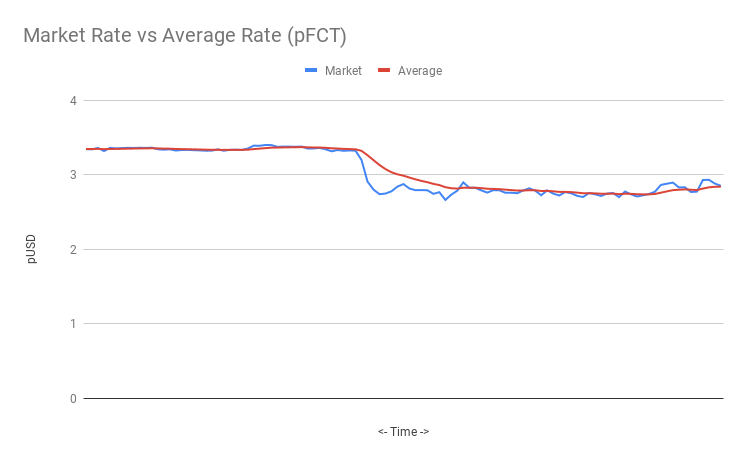
\includegraphics[width=\textwidth]{rategraph.png}
  \caption{You can see how the average price is less affected by swings in the market price.}
\end{figure}


\pagebreak
\subsection{Conversions}
Conversions are how Pegnet handles converting 1 pAsset to another.

    \subsubsection{Simple Calculation}
    
    The simple calculation uses the latest {\bf market rate}. When doing a conversion, there is always a {\bf Source-Asset} and a {\bf Destination-Asset}. For a conversion of a pFCT $\rightarrow$ pUSD, pFCT is the source, and pUSD is the destination. The formula computes the destination amount in the destination units. All rates in the formula are {\bf market rates}.
    
    
    \large{\[
    DestAmount = SourceAmount * \frac{SourceMktRate}{DestMktRate}
    \]}


    \pagebreak
    \subsubsection{Spread}
    
    Pegnet simulates market spread by using a combination of the market and average rate. To do this, we use the same formula as above, but change which rates are used. All rates in the formula are {\bf rate tuples} of market and average rate.
    
    \large{\[
    DestAmount = SourceAmount * \frac{min(SourceRate)}{max(DestRate)}
    \]}
    
    The spread from the market rate can be computed like so:
    \large{\[
    Spread = \frac{SourceMktRate}{DestMktRate} - \frac{min(SourceRate)}{max(DestRate)}
    \]}
    
    The spread is the amount lost in the conversion. Notice the numerator is always min, and the denominator is always max. This means the spread always works against you, it will never benefit a trader. Highly volatile assets will be hit with higher spread.
    
    Examples, with MktRatio being the ratio you'd receive without spread, and PegnetRatio being the amount you'd receive with spread per source asset. So 1 source asset * ratio = destination amount. To get the spread percent, the spread is divided by the MktRatio.
    \begin{center}
    \begin{tabular}{ |c|c|c|c|c| } 
    \hline
    SrcRate (Mkt, Avg) & DstRate (Mkt, Avg) & MktRatio & PegnetRatio & Spread \\
    \hline
    \hline
     (\$5.00, \$4.95)  & (\$1.00, \$1.00) & 5 & 4.95 & 1\% \\ 
    \hline
     (\$2.4112, \$19.5716)  & (\$2.4151, \$19.3165) & 0.12319 & 0.12502 & 1.46\% \\ 
    \hline
    \end{tabular}
    \end{center}

    \pagebreak
    \subsubsection{Spread Tolerance}
    
    Spread is intended to mitigate attacks on the Pegnet in markets with low liquidity. Low liquidity being relative to the upside benefit of an attack. The downside of this mitigation, is that is hits all traders equally in normal operation. To attempt to reduce the impact of spread in most cases, a level of spread tolerance can be introduced. The spread tolerance has the goal of bringing the average rate closer to the market rate. This means the tolerance will never change the market price, it will only ever affect the average price.
    
    To add price tolerance, we use the same price formulas as above, but we expand the $min$ and $max$ parts of the equation. The goal of the tolerance is to reduce the spread, but never give the conversion a discount (negative spread). The $tolerance$ is some fixed percentage of the MktRate.
    
    MinTolerance(rate) will never go above the MktRate, but it will bring the average up until the MktRate. So if the market is bullish, the trailing average will be less than the market, and the tolerance will bring the avg closer to the market rate, increasing the value that you are converting from.
    
    
    \[ MinTolerance = \begin{cases} 
      MktRate & AvgRate \geq MktRate \\
      min(MktRate, AvgRate + tolerance) & MktRate > AvgRate \\
   \end{cases}
    \]
    
    MaxTolerance(rate) will never go below the MktRate, but it will bring the average rate down. So if the market is bearish, the trailing average will be greater than the market, and the tolerance will bring the avg closer to the market rate, decreasing the value that you are converting to (resulting in more tokens purchased).
    \[ MaxTolerance = \begin{cases} 
      MktRate & AvgRate \leq MktRate \\
      max(MktRate, AvgRate - tolerance) & MktRate < AvgRate \\
   \end{cases}
    \]
    
    Calculating the tolerance is done by taking a fixed constant $Volatility Limit$, and multiplying it by the market rate. If the $Volatility Limit$ is 1\%, then the tolerance formula is:
     \[ 
     tolerance = 0.01 * MktRate
    \]
  

\end{document}
